\chapter{REVISIÓN SISTEMÁTICA DE LITERATURA}
\label{ch:revision} % Etiqueta para referenciar en TOC

Este capítulo presenta de manera general una revisión sistemática de la literatura centrada en el fenómeno de la BS y su impacto en la exactitud de los IPS basados en UWB. Dado que la obstrucción causada por el cuerpo humano es uno de los principales factores que degradan el desempeño de estos sistemas, especialmente en aplicaciones de seguimiento de personas, revisar el estado del arte es fundamental para proponer soluciones innovadoras y efectivas.

\section{METODOLOGÍA DE REVISIÓN SISTEMÁTICA DE LITERATURA}
\label{sec:metodologia_revision}

Para asegurar una revisión de la literatura relevante, se llevó a cabo una búsqueda en varias bases de datos académicas, con el fin de identificar los estudios más relevantes sobre el efecto de la BS en los IPS basados en UWB. Las bases de datos seleccionadas fueron: Scopus y Web of Science, ya que estas fuentes proporcionan la mayor cantidad de publicaciones en el campo de la ingeniería y las telecomunicaciones.


\textbf{Palabras clave utilizadas:}

Las palabras clave que guiaron la búsqueda fueron:
\begin{itemize}
    \item \textit{UWB localization.}
    \item \textit{Body Shadowing.}
    \item \textit{Ultra-Wideband Signal Propagation.}
    \item \textit{Indoor Positioning Systems.}
\end{itemize}
Estas palabras clave se combinaron y utilizaron para buscar tanto en los títulos como en los resúmenes de los artículos. Posteriormente, se empleó una estrategia de búsqueda cruzada con las referencias de los artículos encontrados inicialmente para ampliar la cantidad de publicaciones relevantes.

\section{PROCESO DE FILTRADO DE ARTÍCULOS}
\label{sec:filtrado}

Se establecieron criterios de selección específicos para filtrar e identificar los artículos más relevantes en función de los objetivos de la investigación. En una primera etapa, se encontraron 57 artículos. Tras aplicar los criterios de selección y descartar los artículos repetidos, quedaron 20 artículos que abordan específicamente los efectos de la BS sobre la exactitud y exactitud de los IPS basados en UWB, tal como se muestra en la Figura \ref{fig:articulos}.

Los criterios de selección utilizados en la revisión de la literatura científica fueron:
\begin{itemize}
    \item Estudios que analicen IPS basados en UWB como tecnología base.
    \item Estudios que evalúen los efectos de BS en la propagación de señales UWB
    \item Trabajos realizados en escenarios como edificios universitarios, casas, u oficinas.
    \item Estudios basados en experimentos o simulaciones que involucren interacción entre las señales de dispositivos UWB y el cuerpo humano.
    \item Documentos que proporcionen información sobre métodos, resultados y análisis técnico de los sistemas de posicionamiento y la BS.
\end{itemize}
Se definieron también los siguientes criterios de exclusión:
\begin{itemize}
    \item Estudios que no se centren en UWB como tecnología principal; por ejemplo, Bluetooth, WiFi o RFID.
    \item Trabajos en escenarios de exteriores o en escenarios no aplicables al estudio de escenarios de interiores tales como escenarios industriales.
    \item Redes de comunicación enfocadas en aplicaciones específicas diferentes a la localización.
\end{itemize}
%
\begin{figure}[ht]
    \centering
    \includegraphics[width=1\textwidth]{imagenes/diagrama_burbujas_espanol.pdf}
    \caption{Selección y Distribución de Artículos}
    \label{fig:articulos}
\end{figure}

Tras el proceso de filtrado, los 20 artículos seleccionados se organizaron en tres categorías principales según su enfoque metodológico, lo que permite un análisis estructurado del estado del arte. La Figura \ref{fig:articulos}  presenta las categorías mencionadas. La primera categoría corresponde a los estudios basados en simulación, que modelan el impacto de la BS. La segunda agrupa los estudios experimentales, enfocados en la validación empírica en escenarios reales. Finalmente, la tercera categoría reúne los estudios de mitigación de error, que proponen algoritmos para corregir las desviaciones causadas por la BS. 


\subsection{Estudios Basados en Simulación}

Se encontraron cuatro artículos relevantes sobre estudios que emplean simulación para estudiar el efecto de la BS sobre la estimación de ToF en sistemas basados en UWB en escenarios de interiores. Estos trabajos se destacan por modelar los errores que se generan en la estimación de distancia debido a la condición de canal NLOS causada por la presencia del cuerpo humano. Estos artículos analizan las variaciones en ToF introducidas por los fenómenos de reflexión y difracción  en condiciones de BS. %Lo anterior permite analizar el efecto de la BS sobre la exactitud de los IPS.

\subsubsection{Referencias de literatura considerada:}
%
\begin{enumerate}
    \item \textbf{FDTD and Empirical Exploration of Human Body and UWB Radiation Interaction on \gls{tof} Ranging} \cite{Otim2019}: Este estudio utiliza simulaciones basadas en el metodo de Diferencias Finitas en el Dominio del Tiempo (\gls{fdtd}) y medidas experimentales extensivas para explorar cómo la señal UWB en 3990 MHz interactúa con el cuerpo humano en escenarios de interiores y de exteriores, y para diferentes condiciones de canal, i.e., LOS, Cuasi Línea de Vista (\gls{qlos}) y NLOS.
    
    Los autores investigan cómo la BS afecta la estimación de distancia basada en el ToF entre un nodo móvil y un nodo fijo y cómo las condiciones del cuerpo modifican el nivel del campo eléctrico recibido. Aunque no se mide potencia directamente, el análisis relaciona las variaciones del campo eléctrico con variaciones de  ganancia en el receptor.

    La Figura \ref{fig:ganancia_wave} visualiza el fenómeno físico de la BS mediante una simulación que genera un mapa de calor de la intensidad de la señal UWB, donde los colores cálidos (amarillo, ~0 dB) indican una señal fuerte y los fríos (azul oscuro, $<$ -40 dB) representan una atenuación severa. Para entender la figura, se debe notar que la señal se propaga de izquierda a derecha.
    
    \begin{itemize}
        \item En el panel (a), se ilustra una condición de LOS, donde el dispositivo receptor se encuentra frente al cuerpo. Se observa que la señal incidente llega con alta intensidad (color amarillo), sin ser atenuada significativamente.
        \item En el panel (b), se representa una condición de NLOS. Aquí, el cuerpo está girado y bloquea completamente la trayectoria directa de la señal. El dispositivo receptor queda inmerso en la "sombra" de atenuación (color azul oscuro), donde la intensidad de la señal se reduce en más de 40 dB.
    \end{itemize}

    
%%
    \begin{figure}[ht]
    \centering   \includegraphics[width=0.9\textwidth]{imagenes/datos_LOS_NLOS_QLOS.png}
    \caption{Visualización del Fenómeno de Obstrucción Corporal mediante Simulación FDTD en Condiciones LOS (a) y NLOS (b)}
    \label{fig:ganancia_wave}
    \end{figure}

    \item \textbf{Human Body Shadowing Effect on UWB-Based Ranging System for Pedestrian Tracking} \cite{ref16}: Los autores desarrollaron un modelo basado en simulación que predice cómo el error de ToA afecta la estimación de distancia, considerando la interacción entre las señales UWB y el cuerpo humano. El modelo distingue entre la ubicación del nodo móvil en el cuerpo y su orientación con respecto a un nodo ancla fijo.
    Los autores realizaron simulaciones utilizando un modelo geométrico simplificado de un cilindro vertical para representar el torso humano. En su esquema, un nodo ancla se encuentra en el techo y un nodo móvil sobre el cuerpo. Para analizar el efecto de la obstrucción o Ángulo de Orientación Relativo (\gls{rha}), definen el ángulo de orientación corporal, $\theta$, como el ángulo entre la dirección frontal del torso y la línea de visión directa hacia el nodo ancla.

    \begin{figure}[ht]
        \centering   \includegraphics[width=1\textwidth]{imagenes/RHA_ref17.pdf}
        \caption{Posición Relativa entre el Nodo Móvil y el Nodo Fijo (a) Ejemplo 1, (b) Ejemplo 2.}
        \label{fig:posicion_relativa_nodo_fijo_movil}
    \end{figure}

    El estudio clasifica los escenarios de propagación en tres categorías según el RHA o $\theta$, este ángulo mide la orientación del nodo móvil con respecto al nodo fijo: la condición LOS ocurre cuando el RHA es cercano a $0\degree$, lo que significa que la dirección de la caminata se alinea con este eje de referencia (linea punteada) y el cuerpo del peatón queda detrás del dispositivo. En contraste, la condición de NLOS se produce cuando el RHA se aproxima a $180\degree$, indicando que el peatón se mueve en dirección opuesta al ancla, interponiendo su torso como un obstáculo directo. Las zonas de \gls{qlos} representan los estados de transición críticos, que se manifiestan con un RHA cercano a $90\degree$ y $270\degree$, donde la trayectoria de la señal no está ni despejada ni completamente bloqueada, sino que se difracta por los contornos laterales del cuerpo, estas posiciones de la dirección del movimiento de pueden ver en la figura \ref{fig:posicion_relativa_nodo_fijo_movil}. Los experimentos se llevaron a cabo en un escenario de interiores con dimensiones de 13 m $\times$ 83 m $\times$ 2.5 m, evaluando distancias entre transmisor y receptor de 1 a 6 m con un muestreo a 3.5 Hz. Se utilizaron nodos UWB portátiles acoplados al cuerpo de los participantes, quienes presentaban diferencias en altura y peso, i.e., B1: 1.73 m, 77 kg; B2: 1.66 m, 50 kg.
     
    Los resultados del estudio indican que en condiciones de LOS, el error de estimación de distancia presenta un comportamiento estable y de baja dispersión, con una media que varía entre 0.12 m y 0.15 m y una desviación estándar entre 0.09 m y 0.15 m. Este comportamiento se asocia con una distribución aproximadamente gaussiana. En contraste, bajo condiciones de NLOS, este error de estimación de distancia se incrementa significativamente, alcanzando valores medios de hasta 0.5 m y desviaciones estándar de hasta 0.7 m, lo que evidencia una marcada degradación en el desempeño del sistema.

    Un aspecto fundamental del artículo es que no se limita a este modelo binario (LOS/NLOS), sino que analiza los estados de QLOS. Para ello, los autores introducen la métrica del grado de obstrucción, que va de 0 (visión directa) a 1 (obstrucción total). Los resultados muestran cómo el error aumenta progresivamente: con una obstrucción lateral de 0.5, el error medio es de 0.17 m; y con una obstrucción casi completa de 0.8, el error medio sube a 0.36 m, demostrando una relación directa entre el grado de bloqueo y la imprecisión.

    Los autores concluyen que para la condición LOS, i.e., RHA $\approx$ 0, el error es mínimo, con una media de 5.5~cm y una desviación estándar de 3.6~cm. En la zona de transición con, i.e., QLOS y RHA de $\approx 92\degree$ la difracción de la señal por el costado del cuerpo eleva el error a una media de 11.8~cm con una desviación estándar de 4.5~cm. En condición NLOS, i.e., RHA = $180\degree$, la obstrucción total del torso provoca que el error alcance su punto máximo, con una media de 38.9~cm y una desviación estándar de 13.9~cm.

    \item \textbf{Non-Line-of-Sight Identification based on Unsupervised Machine Learning in Ultra Wideband Systems} \cite{Fan2019}: Aunque este estudio se clasifica en simulación, también es relevante en la mitigación del error NLOS mediante técnicas de Aprendizaje Automático (ML, \textit{Machine Learning}) no supervisado, las cuales se utilizan para identificar condiciones de propagación LOS y NLOS en sistemas de localización basados en UWB. 
    
    Para este análisis se realizaron simulaciones en MATLAB utilizando un modelo de canal UWB en un escenario de interiores, generando 1000 formas de onda, de las cuales 500 representaban condiciones LOS y 500 NLOS. A partir de estas señales, se extrajeron tres características clave: número de caminos significativos (NP), retardo en exceso medio ($\tau_{\textrm{MED}}$) y dispersión de retardo RMS ($\tau_{\textrm{RMS}}$). Estas características fueron utilizadas para alimentar un algoritmo de ML  no supervisado basado en Maximización de la Expectativa (EM, \textit{Expectation Maximization}) para Modelos de Mezcla Gaussiana (GMM, \textit{Gaussian Mixture Model}) \cite{ref20}. Un GMM es un modelo probabilístico que asume que los datos pueden representarse como una combinación de varias distribuciones gaussianas (o normales). Cada una de estas distribuciones gaussianas representa un componente de la mezcla y puede describir un subconjunto específico de los datos, es decir, que un GMM asume que cada grupo de datos sigue una distribución normal. 
    %
    %En el caso de este artículo, cada grupo de datos corresponde a las condiciones de canal LOS y NLOS. 
    %
    
    Si bien el estudio no se enfoca exclusivamente en la BS, el enfoque permite clasificar señales LOS y NLOS sin etiquetado manual, un avance importante en la automatización del proceso de identificación de las condiciones de canal. 
    
    Los autores presentan que la clasificación de señales LOS y NLOS tiene una tasa de clasificación correcta del 86.5\%; una tasa de falsos negativos del 12.7\% donde se identifican condiciones LOS cuando en realidad son NLOS; y de falsos positivos del 0.8\% donde se identifican condiciones NLOS cuando en realidad son LOS.
    
    \item \textbf{Modeling, Validation and Performance Evaluation of Body Shadowing Effect in Ultra-Wideband Networks} \cite{Ruonan2019}: Los autores de este estudio modelaron la BS en redes UWB, presentando que este fenómeno introduce pérdidas significativas de señal que dependen de la orientación del cuerpo humano respecto al transmisor y receptor, es decir, de la dirección en la que está orientado el cuerpo en relación con la trayectoria de la señal. Además, los autores proponen un modelo matemático que mejora la exactitud de los resultados de simulaciones y predicciones del comportamiento del canal en presencia de BS.

    Los autores modelaron y simularon los efectos de la BS sobre los sistemas de comunicación UWB en escenarios de interiores, lo cual es clave para mejorar la exactitud en aplicaciones de localización y seguimiento en tiempo real. Para este análisis, los autores emplearon simulaciones basadas en IEEE 802.15.3a que es una propuesta de extensión al estándar IEEE 802.15.3 y que fue cancelada en 2006, pero aun así se reconoce su relevancia como un estándar de facto para simulaciones UWB debido a su capacidad para representar escenarios de interiores bajo distintas condiciones de canal, i.e., LOS y NLOS.

    Aunque el trabajo es de simulación, se incluye una fase de validación que hace uso de medidas  experimentales previamente disponibles.
    
    Las simulaciones consideran un transmisor y un receptor separados por una distancia de 3 m, situados a 1.2 m de altura. El cuerpo humano se modela como una elipse vertical con un ancho de 0.5 m, y se representa como una barrera que bloquea completamente la propagación de la señal UWB en la dirección frontal, es decir, cuando el cuerpo humano se interpone en línea directa entre el transmisor y el receptor. En el estudio, los ángulos se determinan a partir de un modelo geométrico que define la orientación del cuerpo humano en relación con la línea recta entre el transmisor y el receptor. No se utilizaron nodos físicos; en cambio, se calcularon los ángulos de incidencia de la señal sobre el cuerpo para asignar una pérdida de señal proporcional. Esta pérdida es máxima, 20 dB, cuando la señal incide de forma frontal, i.e., 0$^\circ$, y disminuye progresivamente hacia los lados, hasta anularse en direcciones laterales, i.e., $\pm90^\circ$. Esta función de atenuación se implementa como un filtro direccional sobre las trayectorias del canal.
    
    En las simulaciones, el modelo de canal base utilizado es el IEEE 802.15.3a para condiciones de canal de interiores NLOS.  

    Los resultados muestran que, en presencia de BS, la media de la potencia recibida disminuye entre 5 y 15 dB, dependiendo del ángulo de incidencia. Por ejemplo, cuando la dirección de propagación es frontal, i.e.,  0$^\circ$, se observa una atenuación media de 13.2 dB, mientras que para ángulos cercanos a $\pm90^\circ$, la atenuación es casi nula. El impacto sobre el error de estimación de distancia se analiza mediante simulaciones de localización, donde se observó un aumento promedio del error del 35\% en presencia de BS, con errores que pasaron de 0.18 m sin BS a 0.24 m con BS en escenarios NLOS.

    Los autores también evaluaron la Tasa de Paquetes Pérdidos (PER, \textit{Packet Error Rate}) como función de la posición relativa del cuerpo. En el peor caso, i.e., bloqueo completo de la LOS, el PER alcanzó hasta un 70\%, mientras que en ausencia de obstrucción fue inferior al 10\%. Estos resultados validan el modelo direccional propuesto, que incorpora la orientación corporal como un parámetro clave para simular con exactitud los efectos de la BS en sistemas UWB.
\end{enumerate}

\textbf{Contribución}\\
La contribución conjunta de los estudios de simulación es fundamental para modelar el efecto de la BS a través de distintas métricas para las condiciones LOS, NLOS y QLOS. Estos trabajos abarcan un espectro de enfoques que van desde modelos de FDTD, que correlacionan la atenuación del campo eléctrico con el MAE, hasta modelos geométricos-probabilísticos más simples que definen RHA para cada condición y predicen la distribución estadística del error. Además, otros enfoques utilizan la simulación para entrenar algoritmos de ML capaces de clasificar automáticamente el estado del canal basándose en características de la señal, o proponen modelos de atenuación paramétricos para evaluar el impacto en métricas a nivel de sistema, como la Tasa de Paquetes Pérdidos (PER).


\subsection{Estudios Experimentales}

\subsubsection{Referencias de literatura considerada:}

\begin{enumerate}
    %\setcounter{enumi}{3} % Continúa la numeración de la lista anterior
    \item \textbf{Impact of Body Wearable Sensor Positions on UWB Ranging} \cite{ref14}: Este estudio analiza cómo la posición de los nodos ubicados en diferentes partes del cuerpo, específicamente en frente, mano, pecho, muñeca, brazo, muslo y tobillo, afecta la exactitud de la estimación de distancia utilizando tecnología UWB. 
    
    Los autores determinaron que la posición en la frente proporcionaba los mejores resultados en términos de exactitud de localización. Este estudio proporciona información acerca de la ubicación del receptor UWB en el cuerpo humano para aplicaciones de seguimiento de peatones. Los investigadores utilizaron el kit de desarrollo TREK1000 fabricado por Decawave, el cual opera a una velocidad de transmisión de datos de 110 kbps en el canal 2 a una frecuencia de 3990 MHz.

    Los resultados mostraron que la ubicación del nodo móvil en el cuerpo afecta significativamente la exactitud del ToF, lo que repercute en la estimación de distancia. En LOS, el nodo móvil en la frente presentó los mejores resultados con un error medio de 20 cm, seguido de la mano, muñeca, tobillo, brazo, muslo y pecho. En NLOS, los errores aumentaron considerablemente, alcanzando valores de hasta 2.2 m en el pecho debido al multitrayecto. Se observó que en NLOS, la propagación de ondas UWB está dominada por fenómenos de difracción y propagación por ondas rasantes, siendo estas últimas un tipo de propagación de ondas electromagnéticas en la que la señal viaja muy cerca o alrededor de una superficie.

    Para modelar el error de estimación de distancia, se ajustaron distribuciones estadísticas a la distribución de los resultados experimentales. En LOS y QLOS, los errores siguieron una distribución de probabilidad gaussiana, con una media de 13 cm y una desviación estándar de 8 cm para la frente. En NLOS, los errores fueron modelados con una distribución de probabilidad gamma, con valores máximos de 2.08 m, 0.91 m y 0.47 m en el pecho, la muñeca y la mano, respectivamente. Se observó que la relación entre el RHA y el error de distancia no es lineal en algunas ubicaciones, especialmente en el pecho, donde la correlación entre el error medio de distancia y el RHA fue de -0.69, lo que indica una variabilidad moderada.

    \item \textbf{Gaussian mixture model, IMU, UWB, human body shadowing, indoor localization, particle filter} \cite{Tanghe2023}: Este estudio analiza los valores de ToF de una señal UWB por efecto de la BS y cómo esta afecta la estimación de distancias entre nodos y como consecuencia, su efecto sobre la estimación de la localización del nodo móvil haciendo uso de la técnica de trilateración. 
    
    El IPS basado en UWB está conformado por tres nodos ancla y un nodo móvil operando a una frecuencia de 3990 MHz, el cual fue diseñado para el seguimiento de peatones. El estudio se basa en pruebas experimentales en tres escenarios distintos: una oficina de 3.95 m $\times$ 6.15 m, un laboratorio de 10.9 m $\times$ 21.0 m y una cancha de baloncesto al aire libre. Se utilizaron cuatro nodos EVB1000 de Decawave, configurados como nodos ancla (ANC) y nodos móviles (TAG), operando en el canal 2, i.e., 3993 MHz, con una velocidad de transmisión de datos de 110 kbps y una frecuencia de toma de medidas igual a 3.57 Hz. Las medidas se registraron durante 174 minutos, lo que representa más de 37000 medidas de distancia.

    Los resultados muestran que la BS introduce errores sistemáticos en la estimación de ToF, lo que afecta negativamente la exactitud del sistema de localización. Los resultados mostraron que el error de distancia en LOS sigue una distribución de probabilidad gaussiana, con un error medio de 8 cm y una desviación estándar de 6 cm. En NLOS, el error se ajusta mejor a una distribución de probabilidad gamma, alcanzando valores máximos de 1.6 m cuando el cuerpo bloquea completamente la señal.

    \item \textbf{Experimental Evaluation Scheme of UWB Radio Propagation Channel with Human Body} \cite{Pradabphon2019}: Este artículo evalúa experimentalmente cómo el cuerpo humano afecta el canal de propagación de señales UWB en el rango de frecuencia de 3 GHz a 11 GHz. 
    
    Las pruebas experimentales se realizaron en dos rangos de frecuencia específicos: de 3 GHz a 7 GHz y de 7 GHz a 11 GHz. Estas mediciones fueron realizadas con un Analizador Vectorial de Redes (VNA, \textit{Vector Network Analyzer}) para evaluar la pérdida de propagación y la distorsión de la señal UWB por BS, en la banda definida por la Comisión Federal de Comunicaciones (FCC, \textit{Federal Communications Commission}) para sistemas UWB. %Los autores analizaron con medidas en laboratorio el impacto de la BS sobre las pérdidas de propagación y la distorsión sobre la señal. 
    
    En LOS, el coeficiente de correlación entre la señal medida y la señal esperada (teórica) disminuyó de 73.96\% a 33.77\% al aumentar la distancia de 2 m a 10 m, respectivamente. En NLOS, el coeficiente de correlación fue aún menor, reduciéndose de 21.4\% a 9.65\% en las mismas condiciones de separación. La pérdida de propagación en la salida del filtro acoplado aumentó de 57.86 dB a 73.38 dB en LOS, mientras que en NLOS, la pérdida de propagación aumentó de 72.75 dB a 80.32 dB para las distancias dadas. Al utilizar un filtro acoplado óptimo, la pérdida de señal se redujo ligeramente, alcanzando valores de 55.24 dB a 63.95 dB en LOS y de 62.36 dB a 66.03 dB en NLOS.

    \item \textbf{Effects of the Body Wearable Sensor Position on the UWB Localization Accuracy} \cite{ref4}: Este artículo analiza la influencia de la posición de un nodo móvil ubicado en el cuerpo humano sobre la exactitud de la localización de un IPS basado en UWB. 
    
    El nodo móvil se ubicó en la frente, mano, pecho, muñeca, brazo, muslo y tobillo, estimando el error de localización en distintas condiciones de canal: LOS y NLOS. Los autores caracterizaron el RHA del cuerpo respecto a los nodos ancla, lo cual permitió definir la condición de canal: LOS o NLOS. 
    
    Los experimentos se realizaron en el Laboratorio Luis Mercader de la Universidad Pública de Navarra, en un área de 78 m$^2$ (13 m $\times$ 6 m $\times$ 4 m), utilizando los kits UWB TREK1000 de Decawave, configurados a una velocidad de transmisión de datos de 110 kbps y a una frecuencia central de 3990 MHz (canal 2). 
    
    En el escenario de pruebas se dispuso de cuatro nodos fijos dentro del laboratorio, mientras que un participante masculino portó el nodo móvil en diferentes partes del cuerpo y recorrió una trayectoria predefinida con 26 puntos de referencia. Las medidas se tomaron en discreto, i.e., con paradas en cada punto de referencia, y continuo, i.e., movimiento sin interrupciones entre las tomas de medidas.

    El error de localización estimado varió significativamente según la ubicación del nodo móvil en el cuerpo. En LOS, la ubicación en la frente presentó el mejor desempeño, con un error promedio de 20 cm y una desviación estándar de 11 cm, mientras que el pecho presentó el peor desempeño, con errores de hasta 4.5 m en NLOS. Los autores identificaron que el mecanismo de propagación dominante en la frente es la difracción, basándose en la baja variabilidad de los errores de posicionamiento observados en dicha ubicación del dispositivo móvil, incluso en condiciones NLOS. Esta afirmación se apoya en estudios previos como \cite{ref11}, donde se establece que la forma curva de la cabeza favorece la propagación de ondas por difracción más que por transmisión directa o reflexión, lo que facilita la propagación de la señal incluso en NLOS. En contraste, los autores identificaron que el pecho genera la mayor cantidad de multitrayecto, basándose en los altos errores de posicionamiento observados que fueron de hasta 4.5 m en NLOS y en la variabilidad de las mediciones. Estos resultados sugieren una fuerte presencia de multitrayecto, probablemente debida a la geometría frontal del torso, que facilita la reflexión de señales hacia múltiples rutas. Aunque el artículo no presenta directamente la Respuesta al Impulso del Canal (\gls{cir}), la interpretación se fundamenta en los errores registrados y en conocimientos previos sobre propagación en presencia de superficies planas y reflejantes del cuerpo humano. 
    
    Los autores utilizaron el Filtro de Kalman Extendido (\gls{ekf}) para estimar la localización del nodo móvil. Los autores compararon los errores de posicionamiento obtenidos en las distintas ubicaciones del nodo móvil en el cuerpo humano con respecto al error de localización obtenido cuando el nodo móvil se montó en un trípode estático. Los resultados mostraron que la frente proporcionó el mejor desempeño del IPS, con un error medio de 0.20 m y un error de 0.35 m en el percentil 90 (P90). En contraste, el pecho presentó el mayor error, con un error medio de 2.46 m y de 4.04 m en el percentil 90 (P90). Las posiciones del nodo móvil en la mano, tobillo, muñeca y muslo mostraron errores intermedios, con valores de 0.62 m, 0.97 m, 1.14 m y 1.46 m en el percentil 90 (P90), respectivamente. 
    
    Los autores concluyeron que la exactitud de localización en sistemas UWB depende críticamente de la posición del nodo móvil en el cuerpo. La frente es la mejor ubicación en términos de desempeño, con respecto al error de localización del nodo móvil en un trípode, i.e., 0.12 m de error de distancia. El pecho es la peor ubicación, debido a la propagación NLOS y la generación de multitrayecto. Los autores recomiendan explícitamente considerar el efecto de la BS y la posición del nodo móvil sobre el cuerpo humano en el diseño de sistemas de localización, especialmente para aplicaciones de seguimiento de peatones en escenarios de interiores. Además, proponen y validan un enfoque de estimación basado en un EKF, lo cual demuestra una estrategia práctica para mejorar la exactitud de localización. 

    \item \textbf{The Effect of Human-Body Shadowing on Indoor UWB TOA-Based Ranging Systems} \cite{ref18}: Este estudio analizó el impacto de la BS en la exactitud de los sistemas de estimación de distancia basados en UWB utilizando TOA. 
    
    Se realizaron dos campañas de medición en frecuencias desde 3 hasta 5.5 GHz, una en una cámara anecoica y otra en un laboratorio. Los autores estimaron CIR, obtenida a partir de la Transformada Inversa Rápida de Fourier (\gls{ifft}) de los resultados en frecuencia. Los autores implementaron un algoritmo de detección del primer pico de señal basado en un umbral para la estimación del TOA, utilizando umbrales de $-70$, $-80$ y $-85$ dB, observando que un umbral menor permite identificar trayectorias difractadas de la señal antes que la componente directa atenuada. Los autores adicionalmente estimaron la atenuación de la señal causada por la BS, así como los errores en la estimación de distancia. 

    Las mediciones se realizaron con un analizador de redes vectoriales Rohde \& Schwarz ZVB-8, con una resolución temporal de 0.4 ns, i.e., equivalente a una resolución espacial de 12 cm. Se emplearon dos antenas Time Domain Broadspec UWB con una ganancia nominal de 3 dBi y un patrón de radiación omnidireccional. El sujeto de prueba fue posicionado entre el transmisor y el receptor en distintas orientaciones. Se realizaron pruebas con distancias entre 4 m y 7 m, variando la orientación del cuerpo en posiciones paralelas y perpendiculares a la línea de propagación.

    Los resultados mostraron que la atenuación de la señal directa causada por la BS depende tanto de la posición como de la distancia entre antenas. En la cámara anecoica, se observaron diferencias en la atenuación de la señal directa causadas por la ubicación del cuerpo humano respecto a los nodos. Específicamente, cuando el cuerpo estaba cerca del receptor, se estimó una pérdida promedio de 12 dB, y de 9 dB cuando estaba cerca del transmisor, lo cual se obtuvo con una separación entre antenas de 8 m. La diferencia de la atenuación percibida puede atribuirse a la geometría del cuerpo, que ofrece diferentes formas de obstrucción según su orientación y cercanía a cada nodo. Cabe aclarar que en esta configuración experimental ninguno de los nodos se mueve y que el cuerpo se desplaza entre posiciones definidas a lo largo de la trayectoria entre transmisor y receptor. En el laboratorio, la atenuación de la señal directa fue, en promedio, mayor que en la cámara anecoica, debido a la presencia de múltiples superficies reflectantes que provocan condiciones de canal donde el efecto de multitrayecto es más complejo. En este escenario, se observaron valores de atenuación de hasta 15 dB cuando el cuerpo se encontraba bloqueando la línea directa entre los nodos. Además, los resultados mostraron que la posición central del cuerpo entre las antenas generaba la menor atenuación cuando el cuerpo estaba orientado en paralelo a la dirección de propagación. Esta disminución se atribuye a que, en esa orientación y ubicación, la proyección del cuerpo sobre la línea directa es mínima, lo que reduce el efecto de la obstrucción.

    Los autores evaluaron el error de distancia mediante el cálculo del Error Cuadrático Medio (\gls{mse}), considerando dos configuraciones: una con 4 m y otra con 7 m de separación entre antenas. Para la configuración de 4 m, el error RMS fue de 26 cm cuando el cuerpo humano se alineó con la trayectoria de la señal en LOS, y aumentó hasta 46 cm bajo condiciones de fuerte atenuación en condición de canal NLOS. Esta última fue inducida al fijar el umbral de detección (\gls{pt}) en $-70$ dB, lo que limitó la capacidad del sistema para detectar señales difractadas. Cuando el PT se redujo a $-80$ dB y $-85$ dB, el error disminuyó  a 14 cm, ya que fueron detectadas señales indirectas alrededor del cuerpo. En la configuración de 7 m, se obtuvieron errores RMS de 21 cm en LOS y hasta 38 cm cuando hubo BS.

    El análisis mostró tres regiones de comportamiento en función del umbral de detección. En la Región I (PT $< -90$ dB), el error aumentó debido a detecciones falsas causadas por ruido. En la Región II ($-85$ dB $< $ PT $< -70$ dB), los errores fueron mínimos, ya que los caminos difractados alrededor del cuerpo dominaban la estimación del TOA. En la Región III (PT $> -70$ dB), el error aumentó porque el TOA se estimaba sobre la trayectoria indirecta más fuerte en lugar del camino directo atenuado.

    Los autores concluyen que, aunque la obstrucción causada por BS atenúa significativamente la señal LOS, esta condición no genera errores adicionales en la estimación de distancia siempre que el TOA sea detectado correctamente a partir de trayectorias difractadas. El estudio demuestra que una adecuada selección del umbral de detección permite minimizar el error de estimación incluso en presencia de BS. No obstante, en escenarios con baja Relación Señal a Ruido (SNR, \textit{Signal-to-Noise Ratio}), la pérdida del componente directo de la señal causada por la BS puede deteriorar la exactitud del sistema. Finalmente, los autores recomiendan que futuras investigaciones consideren configuraciones dinámicas, en las cuales el movimiento del usuario pueda modificar las condiciones de canal para la propagación de la señal en tiempo real.

    \item \textbf{The Effects of Human Body Shadowing in RF-based Indoor Localization} \cite{Schimtt2019}: Este artículo aborda el impacto de la BS en la exactitud de los IPS basados en RF. 
    
    Se llevaron a cabo experimentos utilizando mediciones de ToF a una frecuencia de operación de 2.4 GHz, considerando diferentes posiciones de un dispositivo móvil en el cuerpo y distintas técnicas de localización. Se analizaron los efectos de la BS en escenarios reales de seguimiento sobre la estimación de distancia (error de distancia) como sobre la localización (error de localización). Los experimentos se realizaron en dos escenarios distintos. En el primer escenario, se llevaron a cabo mediciones en un entorno controlado con un único nodo móvil y un nodo ancla, ubicados a distancias de 10 m, 15 m y 20 m. Se evaluaron tres posturas corporales: el nodo móvil colocado al lado derecho de la cadera, al lado izquierdo y en la espalda, con orientaciones de 0$^\circ$, 45$^\circ$ y 90$^\circ$ respecto al nodo ancla. En el segundo escenario, se evaluó un caso práctico de localización inspirado en situaciones de emergencia, como rescates en edificios. Para ello, se desplegaron 14 nodos fijos UWB en un edificio de oficinas, a lo largo de un recorrido total de 60 m. En este segundo escenario, se probaron dos configuraciones: una configuración ideal con los 14 nodos ancla (tanto interiores como exteriores) activos. Otra configuración degradada con solo 12 nodos ancla activos, específicamente los ubicados en el exterior del edificio. Esto se hizo para simular un escenario de emergencia realista donde se pierde la comunicación con los nodos desplegados dentro del área de rescate.

    Los resultados mostraron que la BS genera un error de estimación de distancia de entre 4 m y 14 m, afectando directamente la exactitud de posicionamiento. En el escenario controlado, el Error  Absoluto Medio (\gls{mae}) en la estimación de distancia fue de 4.03 m para 0$^\circ$, 7.93 m para 45$^\circ$ y 14.04 m para 90$^\circ$, lo que demuestra que el error aumenta considerablemente con el ángulo de orientación o RHA del nodo móvil respecto al nodo ancla. En distancias mayores, el efecto fue aun más pronunciado. En 20 m, el MAE alcanzó 4.10 m a 0$^\circ$, 13.56 m a 45$^\circ$ y 8.8 m a 90$^\circ$, lo que sugiere que, en ciertos casos, el efecto del multitrayecto puede compensar la atenuación por la BS.
%
    En el segundo escenario, el error de localización dependió del algoritmo utilizado. Se compararon cuatro algoritmos: Centroid, NLLS (\textit{Non-Linear Least Squares}), MD-Min-Max y Geo-n. Con los 14 nodos ancla activos, los mejores resultados se obtuvieron con Geo-n (MAE de 1.22 m) y MD-Min-Max (MAE de 1.80 m), mientras que NLLS presentó el error más alto con 4.64 m. Cuando se utilizaron 12 nodos ancla en exteriores, la exactitud se redujo significativamente. En este caso, el MAE aumentó a 2.44 m con Geo-n, 3.70 m con NLLS y hasta 6.58 m con MD-Min-Max. Para las distintas ubicaciones del nodo móvil, se encontró que la mejor ubicación fue en la cadera derecha, con un MAE de 1.25 m utilizando Geo-n, mientras que la peor fue en la espalda con un MAE de 2.91 m.

    El análisis también reveló que la cantidad de nodos ancla visibles afecta directamente la exactitud de la localización. En la configuración con todos los nodos ancla activos (tanto en escenarios de interiores como de exteriores), el promedio de nodos visibles por ciclo de medición fue de 6.46. Mientras que al excluir los nodos ancla en interiores, es decir, aquellos ubicados dentro del edificio y más cercanos al usuario, este número se redujo a 4.61, lo que generó un incremento del error de localización del 28.8\%. En la configuración más adversa, con el nodo móvil en el lado izquierdo de la cadera y únicamente nodos ancla exteriores activos, el número de anclas visibles cayó a 2.56, con un aumento del error de localización del 37.8\% respecto a la configuración de referencia.

    Los autores concluyen que el efecto de BS degrada significativamente la exactitud del IPS basado en ToF. La mejor exactitud se obtuvo utilizando el algoritmo Geo-n con un MAE de 1.22 m en condiciones ideales y 2.44 m en el peor caso. La BS incrementó el error en más de 3 m en algunos casos, dependiendo de la orientación y la cantidad de nodos ancla visibles. Los autores recomiendan que los IPS implementen modelos de corrección adaptativos que consideren la posición del nodo móvil y el número de nodos ancla visibles, con el fin de mitigar los efectos de la BS, la pérdida de visibilidad de anclas y la orientación desfavorable del nodo móvil en escenarios reales.

    \item \textbf{Comparing Ubisense, Bespoon and Decawave UWB Location Systems: Indoor Performance Analysis} \cite{Falcone2012}: Este trabajo compara el desempeño de tres IPS distintos basados en tecnología UWB, desarrollados por los fabricantes Ubisense, Bespoon y Decawave. 
    
    Los autores realizaron un análisis experimental en un escenario industrial con condiciones de LOS y NLOS, evaluando la exactitud en la medición de distancias, el desempeño en la estimación de AoA y el desempeño en la localización tridimensional. Además, se empleó un Filtro de Partículas (\gls{pf}) para mitigar la incertidumbre en las medidas y mejorar la exactitud en la localización de los sistemas.

    El experimento se llevó a cabo en un escenario de 24 m $\times$ 14 m (336 m$^2$) dentro del Centro de Automatización y Robótica de España. Se instalaron seis nodos ancla a alturas de 2.32 m, 2.48 m y 2.60 m para el caso de Ubisense, Bespoon y Decawave, respectivamente. Se designaron 70 puntos de prueba en el área de evaluación, con tres repeticiones de mediciones por sistema. El nodo móvil se situó sobre un banco de pruebas a una altura de 0.76 m , 0.72 m y 0.85 m para Ubisense, Bespoon y  Decawave, respectivamente, con tiempos de medición de 30 segundos por punto y tres repeticiones por sistema, lo que equivale a un total de 2100 segundos de observación experimental por sistema. En la estimación de distancias, los resultados mostraron que Decawave presentó la mejor exactitud, con un error medio de 0.12 m y una desviación estándar de 0.232 m. Bespoon tuvo un desempeño ligeramente inferior, con un error medio de 0.43 m y una desviación estándar de 0.634 m. Ubisense, que emplea Diferencia de Tiempo de Llegada (TDoA, \textit{Time Difference of Arrival}), mostró el peor desempeño, con errores superiores a 10 m en múltiples casos y una desviación estándar de 10.6 m. Se observó que tanto Decawave como Bespoon presentan distribuciones de error simétricas con sesgo positivo debido a NLOS, mientras que Ubisense mostró errores más dispersos e inconsistentes.

    En la evaluación de exactitud de localización se utilizaron los datos de estimación de distancia para calcular la posición del nodo móvil mediante trilateración y PF. Decawave obtuvo la mejor exactitud, con un error de localización medio de 0.49 m, mediana de 0.39 m, RMS de 0.59 m y en el percentil 90 de 1.09 m. Bespoon presentó un error de localización medio de 0.71 m, mediana de 0.58 m y RMS de 0.86 m. Ubisense mostró el peor desempeño en la estimación de posición, con un error de localización medio de 1.93 m, RMS de 2.66 m y un percentil 90 de 5.17 m. Sin embargo, cuando se incorporó información de AoA, la exactitud de Ubisense mejoró significativamente, reduciendo el error de localización medio a 1.10 m y RMS a 1.82 m. El análisis de exactitud haciendo uso de información de ángulo reveló que Ubisense es el único sistema que proporciona estimaciones de AoA utilizando un arreglo de antenas en cada nodo. Se estimaron ángulos de azimut y elevación, obteniendo una exactitud de $\pm5.4^\circ$ en azimut y $\pm10.6^\circ$ en elevación, con una tasa de medición válida del 75.4\%, es decir, solo tres de cada cuatro estimaciones angulares fueron aceptadas como confiables. A pesar de la capacidad de estimación de ángulos, la variabilidad de las mediciones sugiere que el sistema requiere un procesamiento adicional para mejorar su confiabilidad.

    El estudio también incluyó una evaluación del impacto del NLOS y la propagación multitrayecto. Se observó que Decawave y Bespoon presentaron distribuciones de error con asimetrías significativas y presencia de valores atípicos, alcanzando errores máximos de hasta 1.2 m y 2 m, respectivamente, como resultado de obstrucciones físicas y trayectorias reflejadas. Por su parte, Ubisense mostró un comportamiento más errático con errores extremos que superaron los 30 m y una tasa de mediciones inválidas del 70\%. Para mitigar estos efectos, se utilizó un modelo de error basado en distribuciones gaussiana y gamma, incorporando el PF para mejorar la exactitud de la localización. En términos de desempeño en escenarios reales, se observó que Decawave y Bespoon son adecuados para IPS, mientras que Ubisense presentó mayores desafíos debido a su alta variabilidad en las estimaciones de distancia. Aunque la integración de AoA en Ubisense mejoró su desempeño, la cantidad de valores atípicos y la necesidad de infraestructura adicional para mejorar la sincronización limitaron su aplicabilidad en comparación con las soluciones basadas en ToF.

    Los autores concluyeron que los dispositivos Decawave ofrecieron el mejor desempeño en la estimación de distancias y la localización en escenarios de interiores, seguidos de Bespoon, que proporcionó una alternativa viable con un desempeño ligeramente inferior. Ubisense, a pesar de mejorar su desempeño al incluir información de AoA, mostró la mayor variabilidad en las estimaciones y la peor exactitud de localización, lo que sugiere que su implementación requiere procesamiento adicional mediante técnicas de filtrado estadístico o fusión de datos, con el fin de compensar su alta variabilidad y mejorar la confiabilidad de las estimaciones en escenarios industriales.

    \item \textbf{The Effects of the Human Body on UWB Signal Propagation in an Indoor Environment} \cite{ref15}: Este trabajo analiza el impacto del cuerpo humano en la propagación de señales UWB en escenarios de interiores. 
    
    Los autores realizaron mediciones experimentales en una cámara anecoica, un auditorio y una oficina, con el propósito de comparar el efecto de la BS en condiciones de baja y alta dispersión de señales. Se evaluaron tres aspectos clave: la atenuación de la señal, las variaciones en el patrón de radiación y la degradación de la calidad del enlace, con el fin de caracterizar la influencia del cuerpo humano en sistemas de comunicación UWB. 
    
    Las mediciones se realizaron con una antena PulseOn Diamond Dipole en el laboratorio de antenas de la Academia de la Fuerza Aérea de los Estados Unidos. En la cámara anecoica, la antena fue montada en un pedestal giratorio e iluminada con una antena Marconi 1804 log-periódica. Se llevaron a cabo mediciones a frecuencias de 2, 3 y 5 GHz con incrementos angulares de 5$^\circ$, cubriendo el patrón de radiación, es decir, la distribución espacial de la intensidad de la señal emitida por la antena en distintas direcciones. Se observó una asimetría en dicho patrón, con una desviación de $\pm2$ dB atribuida a la interacción con el cableado del sistema. Adicionalmente, se realizaron mediciones en el dominio del tiempo, alimentando la antena con un pulso de duración igual a 50 ps, y se analizó la CIR mediante la Transformada Rápida de Fourier (FFT, \textit{Fast Fourier Transform}). En el análisis espectral de esta respuesta se identificó una resonancia principal en 1.7 GHz, entendida como la frecuencia en la que la antena presenta su mayor eficiencia de radiación, es decir, donde transfiere la mayor parte de la energía emitida o recibida, revelando su comportamiento resonante natural ante pulsos ultra anchos en frecuencia. Aunque el sistema fue alimentado con un pulso extremadamente corto de 50 ps, la duración del impulso observado fue de aproximadamente 600 ps, según se reporta directamente en el artículo. Esta diferencia se debe a que la CIR incluye efectos del sistema como resonancia, dispersión y acoplamiento, que extienden la señal en el tiempo. Por tanto, la duración del impulso observado no refleja únicamente la señal de entrada, sino la respuesta completa del sistema bajo prueba.

    En la segunda fase del estudio, se realizaron mediciones en un auditorio, con el transmisor y el receptor separados 5 m y la antena receptora montada en la cintura del usuario. Para estas pruebas se utilizó un sistema con referencia Time Modulated Ultra-Wideband (TM-UWB) de la empresa PulseOn, que permitió obtener mediciones con resolución temporal de 1.1 ns, lo que posibilita una caracterización exacta de las trayectorias múltiples sin requerir un sistema basado en ToF. Los resultados mostraron que, en un escenario de baja dispersión multitrayecto, i.e., con escasa reflexión y baja densidad de trayectorias indirectas, la BS  generó una atenuación pronunciada al bloquear la señal LOS, lo que se manifestó como un nulo profundo de 23.6 dB en la región angular comprendida entre los 180$^\circ$ y los 210$^\circ$. Este valor corresponde a una reducción de 23.6 dB en la potencia de la señal recibida debido a la BS y no a una variación del patrón de radiación. Esta atenuación fue registrada directamente en el receptor, como una caída abrupta en la intensidad de la señal medida. Además, se observó que la magnitud del nulo dependía significativamente de la orientación relativa del cuerpo respecto a la antena receptora, evidenciando que el desempeño del sistema está estrechamente relacionado con la geometría y el posicionamiento del usuario. Aunque este sistema no emplea ToF ni estima AoA directamente, su alta resolución temporal permite analizar cómo varía la recepción en función de la dirección y la obstrucción, aportando información útil para evaluar condiciones de visibilidad entre nodos.

    En el tercer experimento realizado en un escenario de oficina con alto multitrayecto, i.e., alta dispersión de la señal, la separación entre transmisor y receptor se redujo a 3.14 m debido a las restricciones del espacio. Se observó que el impacto de la BS en la propagación de la señal se redujo significativamente en comparación con los resultados de las pruebas en el auditorio. La máxima atenuación de la señal fue de 6.8 dB, en contraste con los 23.6 dB en el auditorio. Esto sugiere que en entornos densos con multitrayecto, las reflexiones o ecos de la señal pueden compensar parcialmente la atenuación causada por la BS, mejorando la cobertura del sistema UWB.

    Los resultados indican que la BS puede generar atenuaciones de hasta 23.6 dB en escenarios de interiores con baja dispersión multitrayecto, como un auditorio, lo que afecta negativamente la calidad del enlace en condiciones NLOS. Sin embargo, en escenarios con alta densidad de objetos reflectantes, como oficinas, la atenuación fue considerablemente menor: 6.8 dB, debido a la contribución de trayectorias indirectas generadas por la reflexión de la señal. Esta diferencia se explica porque, en escenarios con alta dispersión, los ecos provenientes de múltiples trayectos pueden compensar parcialmente la atenuación de la señal directa. Los autores concluyen que los sistemas UWB pueden beneficiarse en este tipo de escenarios de alta dispersión por multitrayecto, lo que los hace adecuados para aplicaciones de comunicación en escenarios de interiores complejos.

    Los autores recomiendan que futuras investigaciones evalúen modelos de corrección adaptativa para compensar la atenuación sobre la señal causada por la BS en escenarios de baja dispersión. También sugieren analizar el impacto en diferentes configuraciones de antena y la posibilidad de implementar técnicas de diversidad espacial para mejorar la confiabilidad del enlace en presencia de BS. Cabe señalar que, según el estudio, el patrón de radiación de las antenas no se ve afectado directamente por la BS. La degradación del enlace ocurre por obstrucción de la señal directa, no por una modificación del patrón de radiación.

    \item \textbf{Effect of Human Body Shadowing on UWB Radio Channel} \cite{SasakiEffectHumanBody}: Este trabajo analiza el efecto de la BS en la propagación de señales UWB en Redes de Área Corporal (\gls{ban}). 
    
    Los autores realizaron mediciones experimentales en una cámara anecoica para evaluar la atenuación de la señal cuando un nodo móvil está ubicado en diferentes bolsillos del vestido, i.e., bolsillo derecho de la camisa, el bolsillo frontal del pantalón y el bolsillo trasero del pantalón, variando los ángulos de orientación del cuerpo con respecto al receptor. Los autores analizaron la atenuación de la señal en función del RHA, así como el impacto de la polarización cruzada, es decir, la pérdida de señal causada por la desalineación entre la polarización de las antenas en transmisión y recepción. Los autores compararon los resultados en diferentes posiciones del nodo móvil en el cuerpo y con distintos sujetos de prueba.

     Los autores utilizaron un VNA para obtener la CIR, con una antena de transmisión omnidireccional (monopolo) y una antena receptora tipo bocina situada a 3 m de distancia, a una altura de 0.8 m. Las pruebas se hicieron a una frecuencia central de 8 GHz y una potencia de transmisión de 0 dBm. La discriminación de polarización cruzada del transmisor fue de -17.3 dB a 8 GHz, según los datos de calibración presentados en el estudio. Este valor indica la diferencia de nivel entre la señal transmitida en la polarización principal y la que se recibe en polarización cruzada, reflejando así una pérdida por desalineación de polarización entre las antenas. Esta pérdida fue considerada en el análisis de propagación para evaluar su impacto en la atenuación de la señal bajo diferentes orientaciones del cuerpo.

    La atenuación de la señal debida a BS depende de la ubicación del nodo móvil sobre el cuerpo humano y su orientación con respecto a los nodos fijos. Para el caso del bolsillo de la camisa, se observaron mínimos de señal en ángulos cercanos a 150$^\circ$, mientras que para el bolsillo frontal del pantalón la atenuación máxima se produjo a 45$^\circ$. En el bolsillo trasero del pantalón, los niveles de señal fueron más variables, con fluctuaciones entre 10 y 16 dB dependiendo de la orientación del cuerpo. En algunos casos, la señal recibida en presencia de BS fue aproximadamente 3 dB mayor que en condiciones de espacio libre, debido a reflexiones favorables en la superficie del cuerpo humano, que redirigieron parte de la señal hacia la antena receptora.

    Se evaluó el efecto de la frecuencia en la propagación, es decir, cómo se afecta la transmisión y recepción de señales, comparando mediciones a 4 GHz, 8 GHz y 12 GHz, con un ancho de banda de 0.5 GHz. Se encontró que a 4 GHz, la señal varía de manera más uniforme; esto implica que la señal es más estable, mientras que a 8 GHz y 12 GHz, la atenuación se vuelve más dependiente del RHA. Con el incremento de la frecuencia, i.e., disminución de la longitud de onda, se fortalecen los fenómenos de difracción y dispersión de la señal.

    Los autores también compararon mediciones utilizando diferentes anchos de banda: 0.5 GHz y 3 GHz, ambas con una frecuencia central de 8 GHz. Se observó que con un ancho de banda de 0.5 GHz, los mínimos de señal se presentaron en 50$^\circ$ y 280$^\circ$, mientras que con 3 GHz la atenuación significativa ocurrió únicamente en 50$^\circ$. Esto indica que un mayor ancho de banda proporciona una mayor robustez frente a la BS, debido a la ganancia por diversidad de frecuencia, ya que la señal se distribuye en un rango más amplio en frecuencia. Además, el efecto del multitrayecto es menos severo con anchos de banda mayores, lo que favorece una propagación más estable y menos sensible a los desvanecimientos causados por la orientación del cuerpo.

    Para evaluar la variabilidad entre sujetos, los autores realizaron pruebas con 20 personas: 10 hombres y 10 mujeres. Se calculó la desviación estándar y la mediana de la potencia recibida, encontrando variaciones de 10 a 16 dB dependiendo de la orientación del sujeto. Sin embargo, no se identificaron diferencias estadísticamente significativas entre géneros.

    Los autores concluyeron que la BS afecta significativamente la propagación de señales UWB en BAN, generando atenuaciones que dependen tanto de la ubicación del nodo móvil sobre el cuerpo como de su orientación respecto al receptor. Se observó que las frecuencias más altas presentan una mayor atenuación angular, y que el efecto de multitrayecto, junto con fenómenos de difracción alrededor del cuerpo humano, puede permitir que parte de la señal rodee el cuerpo y contribuya al nivel de potencia de la señal recibida. Además, reflexiones en la superficie corporal pueden incrementar puntualmente la potencia recibida. Por ello, los autores recomiendan considerar cuidadosamente la posición de los nodos UWB en BAN y seleccionar apropiadamente tanto la frecuencia de operación como el ancho de banda, para mejorar la calidad del enlace frente a los efectos de la BS.
\end{enumerate}

\textbf{Contribución:}

Los estudios experimentales permiten una validación empírica de los modelos teóricos y ofrecen datos importantes sobre cómo la posición del nodo en el cuerpo humano afecta la exactitud de los IPS basados en UWB. Estos resultados no solo son esenciales para comprender el impacto de la interacción entre el cuerpo y la propagación UWB, sino que también proporcionan una base sólida para mejorar la exactitud de los IPS en aplicaciones reales, tales como el seguimiento de peatones.

\subsection{Estudios Basados en la Mitigación del Error}

En esta categoría se encuentran estudios que se enfocan en identificar y mitigar los errores introducidos por la BS en IPS basados en UWB. En estos estudios se hace procesamiento de señal para extraer y analizar las características de las señales UWB, las cuales alimentan algoritmos de ML y filtrado que buscan identificar y mitigar el impacto de las condiciones NLOS causadas por la BS sobre el desempeño de los sistemas de comunicación y localización.

\subsubsection{Referencias de la literatura considerada}


\begin{enumerate}
    %\setcounter{enumi}{6} % Continúa la numeración de la lista anterior
    \item \textbf{Feature Selection for Real-Time NLOS Identification and Mitigation for Body-Mounted UWB Transceivers} \cite{Ferreira2021}: Este artículo propone un enfoque basado en ML para identificar y mitigar en tiempo real las condiciones NLOS causadas por la BS en transceptores UWB operando a 3990 MHz, puestos en distintas posiciones del cuerpo. 
    
    Los autores extraen características como el rango ToA, la energía total, el número de trayectorias detectadas y parámetros estadísticos como la desviación estándar del retardo y la varianza de amplitud. Estas variables alimentan algoritmos de clasificación como Random Forest, Gradient Boosting, Máquinas de Vectores de Soporte (\gls{svm}) y K-Vecinos más Cercanos (\gls{knn}), los cuales permiten distinguir entre condiciones LOS y NLOS. Esta clasificación posibilita la mitigación del error de distancia en tiempo real, logrando una mejora significativa en la exactitud, especialmente en posiciones como el pecho y el muslo, donde la BS genera mayor afectación.
    
    \item \textbf{NLOS Identification and Mitigation for UWB Localization Systems} \cite{Guvenc}: Este estudio se centra en la identificación de condiciones NLOS en IPS basados en UWB, utilizando un rango de frecuencias no continuo entre 3 y 11 GHz.
    
    El análisis se enfoca en cómo las señales de UWB interactúan con el cuerpo humano y cómo dicha interacción afecta la estimación del ToF, lo que puede introducir errores en la localización. Para mitigar estos errores, los autores emplean un algoritmo de Mínimos Cuadrados Ponderados (WLS, \textit{Weighted least squares}), que asigna distintos pesos a cada observación según su confiabilidad. Este método ajusta la localización minimizando los errores en función de la calidad de los datos. Los resultados experimentales muestran que identificar correctamente las condiciones NLOS mejora sustancialmente la exactitud del sistema, especialmente en entornos con alta dispersión, como oficinas. El artículo sugiere que el algoritmo WLS puede ser especialmente útil en escenarios reales, donde la calidad de las señales puede variar considerablemente debido a la BS.
    
    \item \textbf{Non-Line-of-Sight Identification based on Unsupervised Machine Learning in Ultra Wideband Systems} \cite{Fan2019}: Aunque este estudio se clasifica también como simulación, es relevante en la mitigación del error NLOS mediante técnicas de ML no supervisado. El GMM permite clasificar automáticamente señales en condiciones LOS y NLOS, ayudando a mitigar el impacto de la BS en la exactitud de los sistemas de posicionamiento.

    \item \textbf{Effects of the Body Wearable Sensor Position on the UWB Localization Accuracy} \cite{ref4}: Este estudio no solo analiza cómo la ubicación de un nodo móvil en el cuerpo afecta la exactitud, sino que también implementa y valida una técnica de mitigación para mejorar la estimación de la localización. Los autores realizaron experimentos en un laboratorio, colocando un nodo UWB en diferentes partes del cuerpo (frente, pecho, muñeca, etc.) y registrando el error en condiciones LOS y NLOS. Para mitigar la incertidumbre y estimar la posición final, los autores emplearon un EKF. Los resultados, ya procesados por el EKF, mostraron que la exactitud y precisión dependen críticamente de la ubicación del nodo en el cuerpo humano: la frente fue la mejor posición, con un error medio de 0.20 m y un error en el percentil 90 (P90) de 0.35 m. En contraste, el pecho fue la peor ubicación, con un error medio de 2.46 m y de 4.04 m en el P90, incluso después del filtrado. La contribución de mitigación del error de este trabajo es la validación de un enfoque práctico basado en el EKF, demostrando que es una estrategia viable para mejorar la exactitud, evaluando su efectividad en función de la posición del dispositivo móvil  en el cuerpo.

    \item \textbf{The Effect of Human-Body Shadowing on Indoor UWB TOA-Based Ranging Systems} \cite{ref18}: Este trabajo investiga el impacto de la BS en sistemas de rango basados en ToA y, fundamentalmente, propone y valida una técnica de mitigación basada en el ajuste de parámetros del receptor. Los autores evaluaron la Raíz Cuadrática Media (\gls{rms}) en configuraciones de 4 m y 7 m de separación. Su contribución a la mitigación reside en cómo manejaron las condiciones NLOS: demostraron que un umbral de PT poco sensible, i.e., -70 dB, limita la capacidad del sistema para detectar las señales débiles difractadas alrededor del cuerpo, lo que resulta en un gran error i.e., hasta 46 cm. La técnica de mitigación propuesta consiste en reducir este umbral para hacerlo más sensible, i.e., -80 dB y -85 dB. Al hacerlo, el sistema fue capaz de detectar correctamente la primera señal difractada, reduciendo el error de localización drásticamente a 14 cm. Por lo tanto, el estudio concluye que una adecuada selección del umbral de detección es una poderosa y eficiente técnica de mitigación para minimizar el error en presencia de BS.

    \item \textbf{The Effects of Human Body Shadowing in RF-based Indoor Localization} \cite{Schimtt2019}: 
    Este artículo aborda el impacto de la BS en la localización en interiores y su principal contribución a la mitigación es la evaluación comparativa de diferentes algoritmos de localización para determinar cuál es más robusto frente a los errores inducidos por la BS. En un escenario práctico simulando un rescate en un edificio de oficinas con 14 nodos UWB, los autores compararon el rendimiento de cuatro algoritmos de mitigación: Centroid, mínimos cuadrados no lineales (\gls{nlls}), método geométrico multimencional min-max y método geométrico optimizado. Los resultados demostraron que la elección del algoritmo es crítica. Con todos los nodos activos, Geo-n fue el más efectivo, logrando un MAE de solo 1.22 m, mientras que NLLS presentó un error de 4.64 m. En el peor de los casos i.e., con solo 12 nodos exteriores activos, el método geométrico optimizado mantuvo su superioridad i.e., MAE de 2.44 m, mientras que el método multidimensional falló drásticamente i.e., MAE de 6.58 m. El estudio concluye que la selección de un algoritmo de localización robusto como el Geo-n es una estrategia de mitigación fundamental y recomienda la implementación de modelos de corrección adaptativos.

    \item \textbf{Comparing Ubisense, Bespoon and Decawave UWB Location Systems: Indoor Performance Analysis} \cite{Falcone2012}: Este trabajo compara el desempeño de tres sistemas comerciales de localización UWB en un entorno industrial realista, y su principal aporte a la mitigación es la implementación y validación de un PF para mejorar la exactitud en condiciones reales de LOS y NLOS. Los autores utilizaron los datos de distancia de cada sistema para alimentar el PF, el cual fue diseñado para manejar la incertidumbre y las distribuciones de error no gaussianas típicas del multitrayecto y la obstrucción. Para mejorar aún más la mitigación, el filtro incorporó un modelo de error estadístico basado en distribuciones gaussiana y gamma. Los resultados demostraron la efectividad de este enfoque: el sistema de Decawave, combinado con el PF, logró la mejor exactitud de localización, con un error medio de 0.49 m y una mediana de 0.39 m. La contribución de mitigación es, por tanto, la demostración de que una técnica de filtrado estadístico avanzado es esencial para compensar la alta variabilidad y mejorar la fiabilidad de los sistemas UWB comerciales en escenarios industriales complejos.
\end{enumerate}

\begin{figure}[ht]
    \centering
    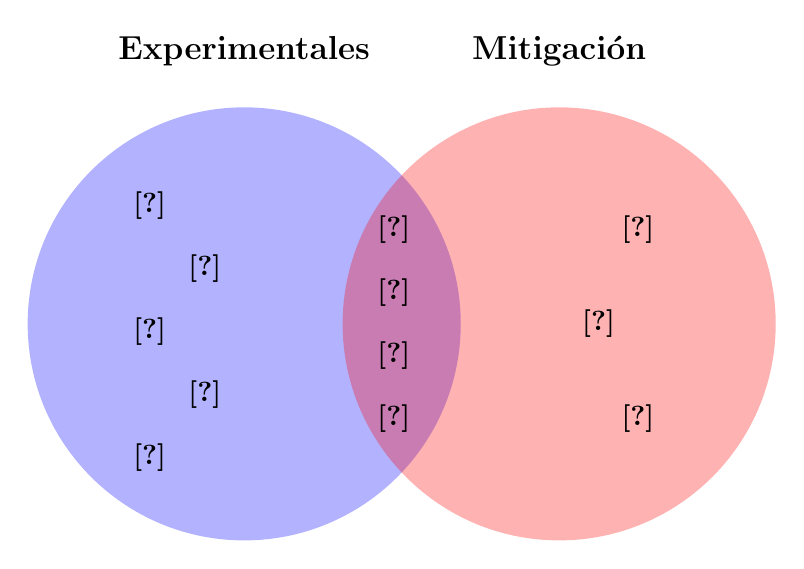
\begin{tikzpicture}[
        % Estilo para los círculos de los conjuntos
        set/.style={circle, minimum size=5.5cm, fill opacity=0.3},
        % Estilo para las etiquetas de los conjuntos
        label/.style={font=\large\bfseries},
        % Estilo para las citas
        citation/.style={font=\bfseries}
    ]
        % --- Dibuja los círculos (conjuntos) ---
        % Círculo para "Estudios Experimentales" (izquierda)
        \node[set, fill=blue] (E) at (-2,0) {};
        
        % Círculo para "Estudios de Mitigación" (derecha)
        \node[set, fill=red] (M) at (2,0) {};

        % --- Coloca los títulos de los conjuntos ---
        \node[label] at ([yshift=0.7cm]E.north) {Experimentales};
        \node[label] at ([yshift=0.7cm]M.north) {Mitigación};
        
        % --- Coloca las citas en sus respectivas zonas ---

        % Zona 1: Solo Experimentales
        % Estas citas se colocan en la parte del círculo azul que no se solapa.
        \node[citation] at (-3.2, 1.5) {\cite{ref14}};
        \node[citation] at (-2.5, 0.7) {\cite{Tanghe2023}};
        \node[citation] at (-3.2, -0.1) {\cite{ref15}};
        \node[citation] at (-2.5, -0.9) {\cite{Pradabphon2019}};
        \node[citation] at (-3.2, -1.7) {\cite{SasakiEffectHumanBody}};


        % Zona 2: Intersección (Estudios Híbridos)
        % Estas citas se colocan en el área de solapamiento.
        \node[citation] at (-0.1, 1.2) {\cite{ref4}};
        \node[citation] at (-0.1, 0.4) {\cite{ref18}};
        \node[citation] at (-0.1, -0.4) {\cite{Schimtt2019}};
        \node[citation] at (-0.1, -1.2) {\cite{Falcone2012}};
        
        % Zona 3: Solo Mitigación
        % Estas citas se colocan en la parte del círculo rojo que no se solapa.
        \node[citation] at (3, 1.2) {\cite{Ferreira2021}};
        \node[citation] at (2.5, 0) {\cite{Guvenc}};
        \node[citation] at (3, -1.2) {\cite{Fan2019}};

    \end{tikzpicture}
    \caption{Clasificación de los Artículos Analizados en Estudios Experimentales, de Mitigación y Estudios Híbridos que Combinan Ambas Metodologías.}
    \label{fig:venn_clasificacion}
\end{figure}

\textbf{Contribución}\\
La contribución fundamental de los estudios de mitigación es el desarrollo y la validación de un diverso ecosistema de técnicas capaces de contrarrestar el error inducido por la BS. Una característica destacada de este grupo de trabajos, como se observa en la figura \ref{fig:venn_clasificacion} es que no son puramente teóricos; la gran mayoría valida sus propuestas a través de implementaciones experimentales, demostrando su aplicabilidad en el mundo real. Estas estrategias de mitigación se pueden agrupar en tres enfoques principales: 1) Clasificación de Canal basada en Machine Learning, donde se emplean algoritmos como SVM, k-NN \cite{ref7} o GMM \cite{ref20} para identificar condiciones LOS/NLOS en tiempo real; 2) Filtrado Estadístico y Estimación de Estados, que utiliza técnicas como Mínimos Cuadrados Ponderados \cite{ref11}, el EKF \cite{ref4} o PF Bayesianos \cite{Falcone2012} para corregir y suavizar las mediciones; y 3) Optimización a Nivel de Sistema, que se enfoca en el ajuste de parámetros del receptor como el PT \cite{ref18} o en la selección del algoritmo de localización más robusto, como Geo-n \cite{ref19}. En conjunto, estos estudios establecen que la mitigación del error por BS es un problema multifacético que puede ser abordado desde el procesamiento de la señal hasta la fusión de datos, proporcionando una caja de herramientas validada experimentalmente para el desarrollo de IPS más precisos y fiables.



\section{ANÁLISIS DE LA REVISIÓN SISTEMÁTICA DE LITERATURA}
\label{sec:analisis_estado_arte}

\subsection{Metodología de la  Revisión}

Para garantizar un proceso de revisión de literatura transparente, riguroso y reproducible, se adoptó la metodología PRISMA (\textit{Preferred Reporting Items for Systematic Reviews and Meta-Analyses}) \cite{PRISMA2020}. PRISMA proporciona una guía basada en evidencia para estructurar la revisión en cuatro fases: Identificación, Cribado (\textit{Screening}), Elegibilidad e Inclusión. Este enfoque documenta el flujo de información desde la búsqueda exhaustiva hasta la selección final de los estudios que conforman el núcleo de este análisis.

\begin{figure}[ht]
    \centering
    \begin{tikzpicture}[
        node distance=1.5cm,
        box/.style={
            rectangle, 
            draw, 
            thick, 
            fill={rgb,255:red,51;green,153;blue,255},
            text=white,
            text width=10cm, 
            minimum height=1.5cm, 
            align=center,
            drop shadow
        },
        arrow/.style={
            -{Stealth[length=3mm]},
            thick
        }
    ]
        % --- Nodos del diagrama ---
        \node[box] (identification) {
            \textbf{Identificación: Registros identificados mediante búsqueda en bases de datos} \\
            (Scopus, WoS) \\
            \textbf{(n = 208)}
        };

        \node[box, below=of identification] (screening) {
            \textbf{Cribado (Screening): Registros únicos tras eliminar duplicados} \\
            \textbf{(n = 204)}
        };
        
        \node[box, below=of screening] (eligibility) {
            \textbf{Elegibilidad: Artículos evaluados a texto completo} \\
            \textbf{(n = 84)}
        };
        
        \node[box, below=of eligibility] (included) {
            \textbf{Inclusión: Estudios incluidos en la síntesis cualitativa} \\
            \textbf{(n = 20)}
        };

        % --- Flechas y texto de exclusión ---
        \draw[arrow] (identification) -- (screening);
        \node[right=0.5cm of screening, text width=4cm, align=left] (dup_removed) {
            Registros duplicados eliminados \\
            \textbf{(n = 4)}
        };
        \draw[arrow] (screening.east) -> (dup_removed.west);
        
        \draw[arrow] (screening) -- (eligibility);
        \node[right=0.5cm of eligibility, text width=4cm, align=left] (screen_excluded) {
            Registros excluidos por título y resumen (no relevantes) \\
            \textbf{(n = 120)}
        };
        \draw[arrow] (eligibility.east) ->(screen_excluded.west);
        
        \draw[arrow] (eligibility) -- (included);
        \node[right=0.5cm of included, text width=4cm, align=left] (fulltext_excluded) {
            Artículos excluidos tras revisión de texto completo \\
            \textbf{(n = 64)} \\
        };
        \draw[arrow] (included.east) -> (fulltext_excluded.west);

    \end{tikzpicture}
    \caption{Diagrama de Flujo PRISMA del Proceso de Revisión Sistemática de Literatura.}
    \label{fig:prisma_flow}
\end{figure}

\subsubsection{Fase de Identificación}
El objetivo de esta fase fue encontrar la mayor cantidad posible de literatura relevante. Se realizaron búsquedas sistemáticas en cuatro bases de datos académicas clave para el campo de la ingeniería y las telecomunicaciones: Scopus y Web of Science (WoS). Se utilizó una combinación de las siguientes palabras clave: UWB localization, Body Shadowing, Ultra-Wideband Signal Propagation e Indoor Positioning Systems. Las bases de datos arrojaron 107 registros y WoS, con 101 registros. Contando todas las fuentes, la búsqueda inicial identificó un total de 208 registros. En esta fase se filtraron los 208 registros. Primero, utilizando software de gestión de referencias Mendeley, se identificaron y eliminaron 4 registros duplicados, quedando así 204 artículos para la fase de cribado o screening. 

\subsubsection{Fase de Cribado (Screening)}
 Los 204 registros únicos restantes fueron sometidos a un cribado basado en título y resumen para excluir aquellos que eran claramente irrelevantes. Se excluyeron 120 artículos en esta etapa por no estar centrados en UWB como tecnología principal, por tratar con aplicaciones distintas a la localización o por enfocarse en escenarios no aplicables.

\subsubsection{Fase de Elegibilidad}
Los 84 artículos que superaron la fase de cribado fueron sometidos a una revisión de texto completo para determinar su elegibilidad final. En esta etapa, se evaluaron en profundidad la metodología, los resultados y el análisis de cada estudio. Se excluyeron 27 artículos adicionales por razones como:
\begin{itemize}
    \item Falta de datos cuantitativos sobre el efecto de la BS.
    \item Metodología experimental no reproducible o insuficientemente descrita.
    \item Enfoque principal en diseño de antenas en lugar de en sistemas de posicionamiento.
    \item Ser resúmenes de conferencias sin un artículo completo disponible.
\end{itemize}

\subsubsection{Fase de Inclusión}
El proceso culminó con la selección de 20 artículos que cumplieron con todos los criterios de inclusión. Estos 20 estudios constituyen la base de la síntesis cualitativa y el análisis del estado del arte presentados en este capítulo. El flujo completo de este proceso se visualiza en el diagrama PRISMA de la Figura \ref{fig:prisma_flow}.
\label{subsec:contexto_analisis}



\subsection{Distribución de Estudios por Tipo de Investigación}
\label{subsec:distribucion_tipos}
%
\begin{figure}[ht]
    \centering
    \includegraphics[width=1.2\textwidth]{imagenes/clasificacion_tipo_investigacion.pdf}
    \caption{Distribución de 20 Artículos por Tipo de Investigación}
    \label{fig:distribucion_tipos}
\end{figure}
%
La Figura \ref{fig:distribucion_tipos} muestra que el 45\% de los estudios son experimentales (9 artículos), seguidos por 35\% de estudios de mitigación (7 artículos) y 20\% de simulación (4 artículos). Esta distribución revela una tendencia marcada hacia la validación práctica de los efectos de la BS, lo cual es fundamental para el desarrollo de sistemas comerciales viables. Los estudios experimentales predominantes incluyen trabajos como \cite{ref4} y \cite{ref14}, que evalúan directamente el impacto de diferentes posiciones del nodo móvil en el cuerpo humano en escenarios controlados.

La proporción relativamente baja de estudios de simulación (20\%) presenta tanto ventajas como desafíos. Por un lado, indica que la comunidad científica prioriza la validación empírica sobre modelos teóricos. Por otro lado, la escasez de simulaciones sofisticadas podría limitar la exploración de escenarios complejos o frecuencias no disponibles comercialmente, como es precisamente el caso de la banda de 6.5 GHz que constituye el foco de esta investigación.

Es importante destacar que esta distribución también refleja la madurez tecnológica del campo. En las etapas iniciales de una tecnología, los estudios de simulación suelen dominar debido a la falta de hardware disponible. Sin embargo, la predominancia actual de estudios experimentales sugiere que la tecnología UWB ha alcanzado un nivel de madurez que permite validación directa, aunque, paradójicamente, esta madurez se concentra principalmente en las bandas de frecuencia inferiores.

\subsection{Frecuencias de Operación Utilizadas en los Estudios}
\label{subsec:frecuencias_operacion}

\begin{figure}[ht]
    \centering
    \includegraphics[width=0.8\textwidth]{imagenes/frecuencias_por_anio.pdf}
    \caption{Distribución de Estudios por Rango de Frecuencia}
    \label{fig:frecuencias}
\end{figure}

La Figura \ref{fig:frecuencias} presenta una concentración abrumadora de investigaciones en las bandas inferiores del espectro UWB. Específicamente, el 70\% de los estudios, i.e., 14 artículos, operan en el rango de 3-5 GHz, mientras que solo el 5\% i.e., 1 artículo, explora frecuencias entre 6 y 7 GHz. Esta distribución no es casual, sino que responde a factores históricos y tecnológicos: la banda de 3.1-5 GHz fue la primera autorizada por la FCC para aplicaciones UWB comerciales, y consecuentemente, la mayoría del hardware disponible opera en este rango.

Solo el 5\% de los estudios analizados operan en frecuencias superiores a 6 GHz. La banda de 6-6.5 GHz permanece prácticamente inexplorada en el contexto de la BS, lo que justifica plenamente el objetivo de esta investigación de analizar el desempeño de sistemas de posicionamiento en 6.5 GHz. Esta frecuencia ofrece ventajas potenciales en términos de resolución espacial mejorada y menor interferencia con otros sistemas de comunicaciones.

La concentración de sistemas en frecuencias bajas tiene implicaciones significativas para el desarrollo futuro de la tecnología. Las frecuencias más altas ofrecen ventajas teóricas importantes, tales como:
%
\begin{itemize}
    \item \textbf{Mayor resolución espacial:} La principal ventaja de UWB es su alta resolución espacial, i.e., la distancia mínima que el sistema puede resolver es del orden de los centímetros, que está determinada por su alta resolución temporal, i.e., pulsos muy angostos del orden de los nanosegundos y que implican un ancho de banda del orden de los 500 MHz. Esta capacidad permite al receptor UWB distinguir con gran exactitud la señal que llega por el primer trayecto o camino directo de los ecos de la misma señal que llegan nanosegundos después. Los sistemas que operan en la banda de 6.5 GHz pueden alcanzar una resolución espacial del orden de centímetros, lo que es fundamental para la localización de alta exactitud y precisión.    
    
    \item \textbf{Menor tamaño de antena:} Las dimensiones de las antenas son proporcionales a la longitud de onda. A 6.5 GHz, las antenas pueden ser aproximadamente 35\% más pequeñas que a 4 GHz, facilitando la integración en dispositivos portátiles.
    
    \item \textbf{Diferentes características de propagación:} Las frecuencias más altas alteran fundamentalmente la interacción de la señal con el entorno. Por un lado, se ha observado que frecuencias mayores, como 8 y 12 GHz, experimentan una atenuación más pronunciada y dependiente del RHA al interactuar con el cuerpo humano en comparación con frecuencias más bajas como 4 GHz \cite{ref19}. Por otro lado, estas mismas frecuencias exhiben patrones de difracción más complejos. Como demuestran estudios en entornos de alta dispersión (como oficinas), estos fenómenos de multitrayecto y difracción pueden ser explotados, ya que los ecos y las señales que rodean el cuerpo pueden compensar la pérdida de la señal directa, mejorando la robustez y la cobertura general del sistema \cite{ref15, ref18}.
\end{itemize}

\subsection{Posiciones del Cuerpo Evaluadas}
\label{subsec:posiciones_cuerpo}
%
\begin{figure}[ht]
    \centering  \includegraphics[width=0.8\textwidth]{imagenes/posiciones_cuerpo.png}
    \caption{Distribución de Estudios por Posición del Nodo Móvil en el Cuerpo Humano}
    \label{fig:posiciones}
\end{figure}
%
La Figura \ref{fig:posiciones} presenta un diagrama radar que ilustra la frecuencia con la que diferentes posiciones corporales han sido evaluadas en la literatura. El pecho y la muñeca emergen como las ubicaciones más estudiadas i.e., 18\% cada una, seguidas por la frente i.e., 15\%. Esta preferencia se debe a consideraciones prácticas: el pecho representa el peor escenario en términos de BS, con errores de localización reportados de hasta 4.5 $m$ en condiciones NLOS \cite{ref4}, mientras que la muñeca simula dispositivos \textit{wearables} comunes como relojes inteligentes.

El análisis detallado de las posiciones revela patrones interesantes:
%
\begin{itemize}
    \item \textbf{Pecho (18\%):} Representa el caso más desafiante debido a la máxima BS. Los estudios como \cite{ref4} reportan errores de hasta 4.5 m en condiciones NLOS cuando el nodo se ubica en esta posición.
    
    \item \textbf{Muñeca (18\%):} Popular debido a la proliferación de dispositivos \textit{wearables}. Sin embargo, esta posición presenta alta variabilidad debido al movimiento natural del brazo durante la marcha.
    
    \item \textbf{Frente (15\%):} Consistentemente muestra el mejor desempeño, con errores típicos de 20 cm en LOS según \cite{ref14}. La forma curva de la cabeza favorece la difracción de señales UWB.
    
    \item \textbf{Posiciones subrepresentadas:} El brazo (8\%), muslo (7\%) y espalda (2\%) han recibido atención marginal, a pesar de su relevancia en aplicaciones específicas.
\end{itemize}

Esta distribución heterogénea sugiere la necesidad imperante de estudios exhaustivos e integrales que evalúen sistemáticamente múltiples posiciones del nodo móvil en el cuerpo humano bajo las mismas condiciones experimentales, permitiendo comparaciones directas y la identificación de patrones.

\subsection{Técnicas de Mitigación Empleadas}
\label{subsec:tecnicas_mitigacion}
%
\begin{figure}[ht]
    \centering
    \includegraphics[width=1.2\textwidth]{imagenes/tecnicas_mitigacion.pdf}
    \caption{Técnicas de Mitigación de Error NLOS}
    \label{fig:mitigacion}
\end{figure}
%
La Figura \ref{fig:mitigacion} ilustra mediante un gráfico polar la distribución de técnicas empleadas para mitigar los efectos de la BS. El análisis revela tendencias significativas en los enfoques adoptados:

\subsubsection{Aprendizaje Automático (43\%)}

Las técnicas de ML dominan el panorama con 6 estudios, reflejando la tendencia actual hacia soluciones basadas en datos. Estas técnicas incluyen:

\begin{itemize}
    \item \textbf{Clasificadores supervisados:} Random Forest, SVM y Gradient Boosting, como en \cite{ref7}, que logran tasas de clasificación LOS/NLOS superiores al 85\%.
    
    \item \textbf{Aprendizaje no supervisado:} GMM con algoritmo EM, como en \cite{ref20}, que permite identificación de NLOS sin etiquetado manual previo.
    
    \item \textbf{Redes neuronales:} Aunque menos comunes, algunos estudios exploran arquitecturas profundas para capturar relaciones no lineales complejas.
\end{itemize}

\subsubsection{Filtros Estadísticos (43\%)}

Representan soluciones más tradicionales pero efectivas:\\

\textbf{A. Filtros de ponderación y partículas}
\begin{itemize}
    \item \textbf{Mínimos Cuadrados Ponderados (WLS):} Como en \cite{ref11}, asignan pesos según la confiabilidad de cada medición.
    
    \item \textbf{Filtros de partículas (29\%)} Utilizados en \cite{Falcone2012} para manejar distribuciones no gaussianas en NLOS.
    
    \item \textbf{Estimadores robustos:} son técnicas estadísticas avanzadas que se utilizan para mejorar la exactitud de los sistemas de posicionamiento UWB. Su función principal es identificar y minimizar el impacto de mediciones extremadamente erróneas (outliers).
\end{itemize}


\textbf{B. Filtro de Kalman (14\%)}\\

Sorprendentemente subutilizado considerando sus ventajas:

\begin{itemize}
    \item Eficiencia computacional superior a la de técnicas de ML.
    \item Capacidad de fusión de datos multinodo.
    \item Predicción de estados futuros útil para seguimiento  continuo.
    \item Implementación madura y bien documentada.
\end{itemize}

Esta subutilización presenta una oportunidad significativa, especialmente para sistemas embebidos con recursos limitados operando a 6.5 GHz.

\subsection{Evolución Temporal de las Investigaciones (2019-2024)}
\label{subsec:evolucion_temporal}
%
\begin{figure}[ht]
    \centering
    \includegraphics[width=1.1\textwidth]{imagenes/evolucion_temporal.pdf}
    \caption{Evolución Temporal de Investigaciones sobre Obstrucción Corporal en UWB}
    \label{fig:temporal}
\end{figure}
%
La evolución temporal presentada en la Figura \ref{fig:temporal} revela patrones interesantes que merecen un análisis detallado:

\subsubsection{Fase de Crecimiento (2019-2022)}

El período 2019-2022 muestra un crecimiento exponencial, con factores catalizadores clave:

\begin{itemize}
    \item \textbf{2019:} Apple introduce el chip U1 en iPhone 11, democratizando el acceso a tecnología UWB.
    \item \textbf{2020:} La pandemia de COVID-19 impulsa la demanda de soluciones de distanciamiento social basadas en localización exacta.
    \item \textbf{2021:} Estandarización IEEE 802.15.4z mejora la seguridad y exactitud en la estimación de distancia de  UWB.
    \item \textbf{2022:} Pico de investigación con 6 estudios, incluyendo primeras exploraciones en frecuencias superiores.
\end{itemize}

\subsubsection{Fase de Consolidación (2023-2024)}

La aparente disminución no indica pérdida de interés, sino una transición hacia:

\begin{itemize}
    \item Investigación más especializada y profunda.
    \item Desarrollo de productos comerciales basados en hallazgos previos.
    \item Exploración de nuevas bandas de frecuencia, como 6.5 GHz.
    \item Integración con otras tecnologías, tales como 5G y WiFi 6E.
\end{itemize}



%%________

\section{ANÁLISIS Y DISCUSIÓN DE LOS HALLAZGOS DE LA REVISIÓN SISTEMÁTICA DE LITERATURA}
\label{sec:analisis_discusion}

\subsection{Síntesis de Hallazgos Principales}
\label{subsec:sintesis_hallazgos}

El análisis de la revisión sistemática de literatura sobre BS en IPS basados en UWB revela un campo de investigación con desarrollo asimétrico. Mientras que las frecuencias entre 3 y 5 GHz han sido exhaustivamente caracterizadas, existe un vacío significativo en el conocimiento sobre el comportamiento de las señales UWB en frecuencias superiores a 6 GHz. Esta disparidad no es meramente académica; tiene implicaciones profundas para el desarrollo futuro de sistemas de localización más exactos, precisos y robustos.

\subsection{Impacto Cuantificado de la Obstrucción Corporal}
\label{subsec:impacto_bs_cuantificado}

Los estudios de simulación han establecido que la BS introduce atenuaciones que varían entre 12 y 20 dB en condiciones de NLOS, con errores de posicionamiento que pueden alcanzar los 60 cm en los peores escenarios. El trabajo en \cite{ref17} utilizando FDTD reveló un fenómeno particularmente intrigante: en condiciones NLOS severas, se observan aparentes "ganancias" de señal de hasta 18 dB debido a la interferencia constructiva entre componentes multitrayecto, principalmente causadas por difracción alrededor del cuerpo humano. Este hallazgo desafía las concepciones simplistas sobre la propagación de señales y subraya la complejidad del fenómeno.

La validación experimental de estos modelos ha confirmado que la posición del nodo en el cuerpo humano es crítica para el desempeño de un sistema de localización. La frente emerge consistentemente como la ubicación óptima, con errores típicos de 20 cm en condiciones LOS que se degradan solo hasta 35 cm en NLOS, representando un incremento del 75\%. En contraste, nodos ubicados en el pecho pueden experimentar degradaciones de hasta 900\%, con errores que saltan de 45 cm en LOS a 450 cm en NLOS. Esta variabilidad extrema entre ubicaciones corporales sugiere que no existe una solución única para todas las aplicaciones, sino que cada caso de uso requiere una evaluación cuidadosa de la ubicación óptima del nodo.

\subsection{Evolución de las Técnicas de Mitigación}
\label{subsec:evolucion_mitigacion}

El panorama de las técnicas de mitigación está dominado por el ML, empleado en el 43\% de los estudios analizados. Algoritmos como Random Forest y SVM han demostrado capacidades impresionantes, alcanzando exactitudes de clasificación LOS/NLOS superiores al 90\%. Sin embargo, esta mejora conlleva costos computacionales significativos que pueden ser prohibitivos para sistemas embebidos con recursos limitados. Además, estos modelos entrenados en frecuencias específicas no son fácilmente transferibles a nuevas bandas de operación, lo que representa un desafío particular para la exploración de la banda de 6.5 GHz.

Los filtros estadísticos tradicionales, aunque menos glamorosos, ofrecen un balance pragmático entre efectividad y eficiencia computacional. El método de Mínimos Cuadrados Ponderados (WLS) ha demostrado reducciones del error RMSE de hasta 45\% con complejidad computacional lineal, siendo atractivo para implementaciones en tiempo real. Sorprendentemente, el EKF, a pesar de su probada eficacia en sistemas de navegación durante décadas, representa solo el 14\% de las implementaciones en la literatura revisada. Esta subutilización presenta una oportunidad significativa, especialmente considerando que el KF ofrece capacidades nativas de predicción de estados y fusión multinodo que son ideales para el seguimiento continuo de personas en movimiento.

\subsection{La Promesa Inexplorada de 6.5 GHz}
\label{subsec:promesa_65ghz}

La migración hacia frecuencias superiores no es simplemente una progresión incremental; representa un cambio cualitativo en las características de propagación que podría revolucionar la mitigación de la BS. A 6.5 GHz, la longitud de onda se reduce a 4.6 cm comparada con 7.5 cm a 4 GHz, lo que implica una mejora del 38.3\% en la resolución espacial teórica. Esta mejora en resolución permite una discriminación más exacta entre componentes de señal directa y multitrayecto, facilitando la identificación del primer pico de señal incluso en condiciones desafiantes.

Paradójicamente, la mayor atenuación corporal esperada a 6.5 GHz podría ser ventajosa para la detección de la condición NLOS. Con una atenuación teórica 30\% mayor que a 4 GHz, las señales que atraviesan el cuerpo serán más claramente distinguibles de aquellas que lo rodean por difracción, simplificando potencialmente los algoritmos de clasificación LOS/NLOS. Además, el coeficiente de difracción mejorado en un 8.2\% sugiere que las señales podrán ``envolver'' el cuerpo más efectivamente, reduciendo las zonas muertas y mejorando la cobertura general del sistema.

\subsection{Limitaciones Sistemáticas en la Literatura Actual}
\label{subsec:limitaciones_sistematicas}

La consideración hacia frecuencias bajas en la literatura no es accidental sino estructural, derivada de la disponibilidad histórica de hardware y la inercia regulatoria. Esta consideración ha creado un círculo vicioso donde la falta de datos experimentales en frecuencias superiores desalienta el desarrollo de hardware, que a su vez limita la investigación experimental. El 95\% de los estudios concentrados en la banda 3-5 GHz han creado una base de conocimiento robusta pero estrecha de conocimiento que no puede extrapolarse confiablemente a frecuencias superiores debido a las diferencias fundamentales en los mecanismos de propagación.

La fragmentación metodológica representa otra limitación crítica. Los estudios típicamente evalúan solo 2-3 posiciones del nodo móvil en el cuerpo humano, como se muestra en la sección \ref{subsec:posiciones_cuerpo}. La mayoría de los estudios se limitan a estudiar típicamente una combinación de pecho, muñeca y frente utilizando protocolos experimentales divergentes, lo que hace imposibles las comparaciones directas. Esta fragmentación se extiende a los escenarios de prueba, donde el 70\% de los experimentos se realizan en laboratorios controlados que no capturan la complejidad de entornos reales con múltiples personas, mobiliario metálico y fuentes de interferencia electromagnética.

\subsection{Oportunidades de Innovación y Contribución}
\label{subsec:oportunidades_contribucion}

Esta investigación se posiciona estratégicamente para abordar estas limitaciones mediante un enfoque metodológico. La evaluación sistemática de seis posiciones del nodo móvil en el cuerpo humano bajo condiciones experimentales idénticas en un aula universitaria real proporcionará el primer conjunto de datos verdaderamente comparable para análisis cruzado. Más allá de llenar brechas de datos, este trabajo establecerá un protocolo experimental reproducible que podrá servir como estándar de facto para futuras investigaciones.

La caracterización estadística del error de posicionamiento por BS en un IPS basado en UWB a 6.5 GHz  representará una contribución fundamental al campo. Esta caracterización no solo incluirá las distribuciones de probabilidad para errores de posicionamiento en condiciones LOS y NLOS. La validación experimental en un escenario real con alta densidad de ocupación y complejidad electromagnética asegurará que los resultados sean directamente aplicables al desarrollo de productos comerciales.

\subsection{Implicaciones para el Futuro del Campo de Investigación}
\label{subsec:implicaciones_futuro}

El impacto anticipado de esta investigación se extiende más allá de las contribuciones técnicas inmediatas. En el corto plazo, los resultados obtenidos permitirán a la academia e industria tomar decisiones informadas sobre aplicaciones e inversiones en tecnología de 6.5 GHz. La caracterización del comportamiento del sistema de posicionamiento favorecerá el desarrollo de chips, tarjetas y reducirá el tiempo de llegada al mercado de productos de próxima generación. En el mediano plazo, se espera que estos hallazgos influyan en la evolución de estándares como IEEE 802.15.4ab, proporcionando resultados empíricos base para decisiones de diseño de protocolos y aplicaciones.

A largo plazo, esta investigación podría catalizar un cambio de paradigma del concepto de los IPS. La demostración de ventajas significativas a 6.5 GHz podría impulsar la exploración de frecuencias aún más altas, incluyendo las bandas milimétricas donde la exactitud subcentimétrica podría ser alcanzable. Además, la metodología desarrollada para caracterización sistemática de la BS podría aplicarse a otras tecnologías de localización emergentes, desde WiFi 6E hasta las futuras redes 6G.

\subsection{Conclusión}
\label{subsec:conclusion_analisis}

El estado actual de la literatura revela un campo maduro en ciertos aspectos, pero con oportunidades significativas sin explotar. La concentración de investigación en frecuencias bajas ha creado una base sólida de conocimiento que ahora debe expandirse hacia nuevas bandas de frecuencia. La banda de 6.5 GHz representa no solo una frontera técnica sino una oportunidad para repensar fundamentalmente cómo se aborda el desafío de la BS en los IPS basados en UWB. 

Esta investigación se posiciona en la intersección crítica entre la necesidad académica de expandir el conocimiento fundamental y la demanda industrial de soluciones prácticas para sistemas de próxima generación. Al abordar sistemáticamente las limitaciones identificadas en la literatura actual y explorar las oportunidades únicas de la banda de 6.5 GHz, este trabajo no solo llenará brechas existentes sino que establecerá nuevas direcciones para la investigación futura en IPS basados en UWB.

%%________